\documentclass[10pt, twocolumn, twoside]{article}
\usepackage[T1]{fontenc}
\usepackage{cuted}
\usepackage{graphicx}
\usepackage{bm}
\usepackage{geometry}
\usepackage{bbm}
\geometry{a4paper,total={170mm,257mm},left=20mm,top=20mm,}
\pagenumbering{arabic}
\usepackage{hyperref}
\usepackage{url}
\usepackage{scrextend}
\usepackage{amsmath,amssymb}
\usepackage{ragged2e}
\usepackage{xcolor}
\usepackage{dirtytalk}
\setcounter{tocdepth}{1}
%\usepackage[backend=biber,style=nature,sorting=nyt]{biblatex}
%\addbibresource{su4.bib}

\title{Quantum Monte Carlo Simulations of the Hubbard model}
\author{Francisco Monteiro de Oliveira Brito}
\date{\today}
\setlength\columnsep{1em}

\makeatletter

\begin{document}

\begin{strip}
\vspace*{\dimexpr-\baselineskip-\stripsep\relax}
\centering
\maketitle
\vskip\baselineskip
\noindent%\makebox[\textwidth]{\rule{1.1\paperwidth}{0.4pt}}
\vskip\baselineskip
\justify
\begin{abstract}\paragraph{}
The interactions between the electrons in a solid give rise to effects that arise specifically due to the many-body nature of the system. The Hubbard model is a minimal model that encapsulates electron correlations, going beyond the periodic ionic potential perturbation or tight binding approach leading to band theory by adding the simplest possible interaction term to a tight binding Hamiltonian. It allows us to make predictions about how properties like magnetism and superconductivity arise and how metal-insulator transitions occur.
\end{abstract}
\end{strip}

\section{Introduction}\paragraph{}

The Hubbard model appeared in 1963 as one of the first attempts to include electron correlation effects in a quantum mechanical description of a solid. Originally, it was introduced to explain the behavior of the electrons occupying the narrow, partially filled $d-$bands of transition metals. Correlation phenomena in these bands lead to a behavior reminiscent of the atomic picture of a solid. We have come a long way since the introduction of the Hubbard model and it is now as paradigm-defining in many-body physics as the Ising model in statistical physics.

These notes aim to present the basic aspects of a numerical technique used to simulate the Hubbard model in a self-contained, tutorial form. The idea is to reduce our problem to solving a set of integrals, which we evaluate numerically through a standard stochastic procedure, known as the Monte Carlo method. These integrals are arrived at upon formulating the quantum many-body description of the system using the Schr\"odinger equation in imaginary time. Hence the name Quantum Monte Carlo.

When Hubbard's seminal paper came out, it followed a trend that arose in the 1950's when people were working on a theory of correlation effects in the free electron gas. Hubbard devised a simple model for the seemingly intractable problem of \emph{interacting} electrons in a band. His work explained qualitatively some properties of transition and rare-earth metals in which electron correlations are non negligible. It turns out that the mathematical formulation of the interaction problem for electrons in a band is not prohibitively complicated, and is perhaps even more amenable to simple computations after some reasonable approximations are introduced. Notably, it is particularly adapted to computer simulations because of its simple approximate Hamiltonian. Moreover, it has been shown to be very relevant in the description of high $T_c$ superconductors. The Hubbard model is clearly very relevant; nonetheless, even the simplified picture it offers is in general difficult to approach analytically. There exists an exact solution in one dimension via Bethe ansatz, but the more general higher dimensional case is often solved numerically. This is the approach we will follow.

Our goal is to apply a QMC technique to simulate electron correlations in a transition metal dichalcogenide (TMD) nanoribbon, a two-dimensional nanostructure made out of some graphene-like compound. The structure is much longer on one direction than on the other, resembling a ribbon, hence its name. The electronic states that accumulate on the edges of this ribbon might lead to interesting magnetic behavior in these TMD nanostructures and this possibility remains unexplored numerically. Moreover, there is some interest in exploring the phase diagram of these systems because recent studies point at the possibility of topological superconductivity. To summarize, we aim to study a two-dimensional strongly correlated graphene-like nanostructure using QMC, a state of the art, unbiased numerical method that allows one to capture the elusive effects of electron correlations.

\section{Hubbard model}\paragraph{}

We start with an overview of the Hubbard model and in section \ref{hubbQMC} we provide details on how to simulate it numerically using quantum Monte Carlo. In particular, we discuss the original motivation to introduce the model and show how the Hubbard Hamiltonian arises as an approximate representation of the Coulomb repulsion between electrons. Finally, we present exact solutions for particular limiting cases, which can be used to crosscheck our simulations.

The nearly free electron gas models the conduction bands of metals and alloys fairly accurately. The high mobility of the electrons compared to the ions justifies an approximate treatment that may be approached in two equivalent ways. The first idea is to treat the periodic potential created by the \emph{virtually} fixed ions (compared to the electrons) as a perturbation on the free electron gas. Another way of arriving at similar results is to imagine that conduction electrons hop from atom to atom. Both these approaches lead to band theory, a framework which allows us to predict whether a material is a conductor or a insulator. The atomic energy levels are broadened, and the electron in the solid occupy energy bands. The highest energy partially filled band is called the conduction band, since it is the band that conduction electrons hopping from atom to atom occupy. However, in transition and rare-earth metals, in addition to the conduction bands, there are partially filled $d-$ or $f-$bands which are responsible for the characteristic properties of these solids. Some of these properties are not explained by band theory, namely the Mott metal-insulator transition.

Take Molybdenum, a transition metal. Its electronic configuration is $[Kr] 4d^5 5s^1$. The $s$-orbital is higher in energy than the $d$-orbital. Thus, the corresponding partially filled band is closer to the Fermi energy. It is then the conduction band. However, the $d$-band will be only partially filled as well, leading to the effects mentioned in the previous paragraph. In Gadolinium, for which the electronic configuration is $[Xe] 4f^7 5d^1 6s^2$, the $d$-level will broaden and correspond to a conduction band when in a solid. However, the partially filled $f$-level will also broaden into a lower energy partially filled band. Platinum is yet another example, with electronic configuration $[Xe]4f^{14} 5d^9 6s^1 $, where the $5d$ level in only partially filled. In these partially filled narrow energy bands correlation phenomena are particularly relevant, as opposed to the case of conduction bands. Thus, the nearly free electron gas model does not suffice to describe the electrons in these bands; we must turn to a model that includes correlations. While for $f-$electrons of rare earth metals, a purely atomic, localized model - such as the Heitler-London model - might be satisfactory, the same cannot be said for $d-$electrons of transition metals because the band they occupy is narrower and correlations should be more relevant since the electronic states within the band are closer in energy.

\subsection{Electron correlations in narrow $d-$bands}\paragraph{}

First, note that the effects of correlations cannot possibly be the same in narrow energy bands and in the nearly free electron gas. To see this, we may simply  recall the shape of a $d-$wave function. In a $d-$orbital, the electron charge density is concentrated near the nucleus. In a solid the electronic charge density should then also be concentrated near the nuclei, as long as the atomic description is useful, even if not completely correct\footnote{The electronic charge density is, of course, not actually defined in terms of a squared norm of the $d-$wave function for a narrow band. There is some broadening of the corresponding atomic energy level, and the wave function describing an electron is a Bloch wave function. Since the band is narrow, we assume that the atomic wave function description is still somewhat useful in a given range and we use it to provide a heuristic motivation for the non validity of the free electron assumption.}. It is much smaller between atoms so that electrons do seem to belong to individual atoms in some sense. For a $d-$band, we assume that the case is not so different since the band is narrow. The fact that we may speak with some meaning of an electron belonging to a particular atom motivates an atomic description, in spite of the fact that the bandwidth of a $d-$band is still appreciable. The point is that electrons in $d-$bands are certainly not well described by a free electron gas, which cannot possibly account for atomic-like behavior.

\begin{figure}[ht!]\label{fig:hydrogenWF}
\centering
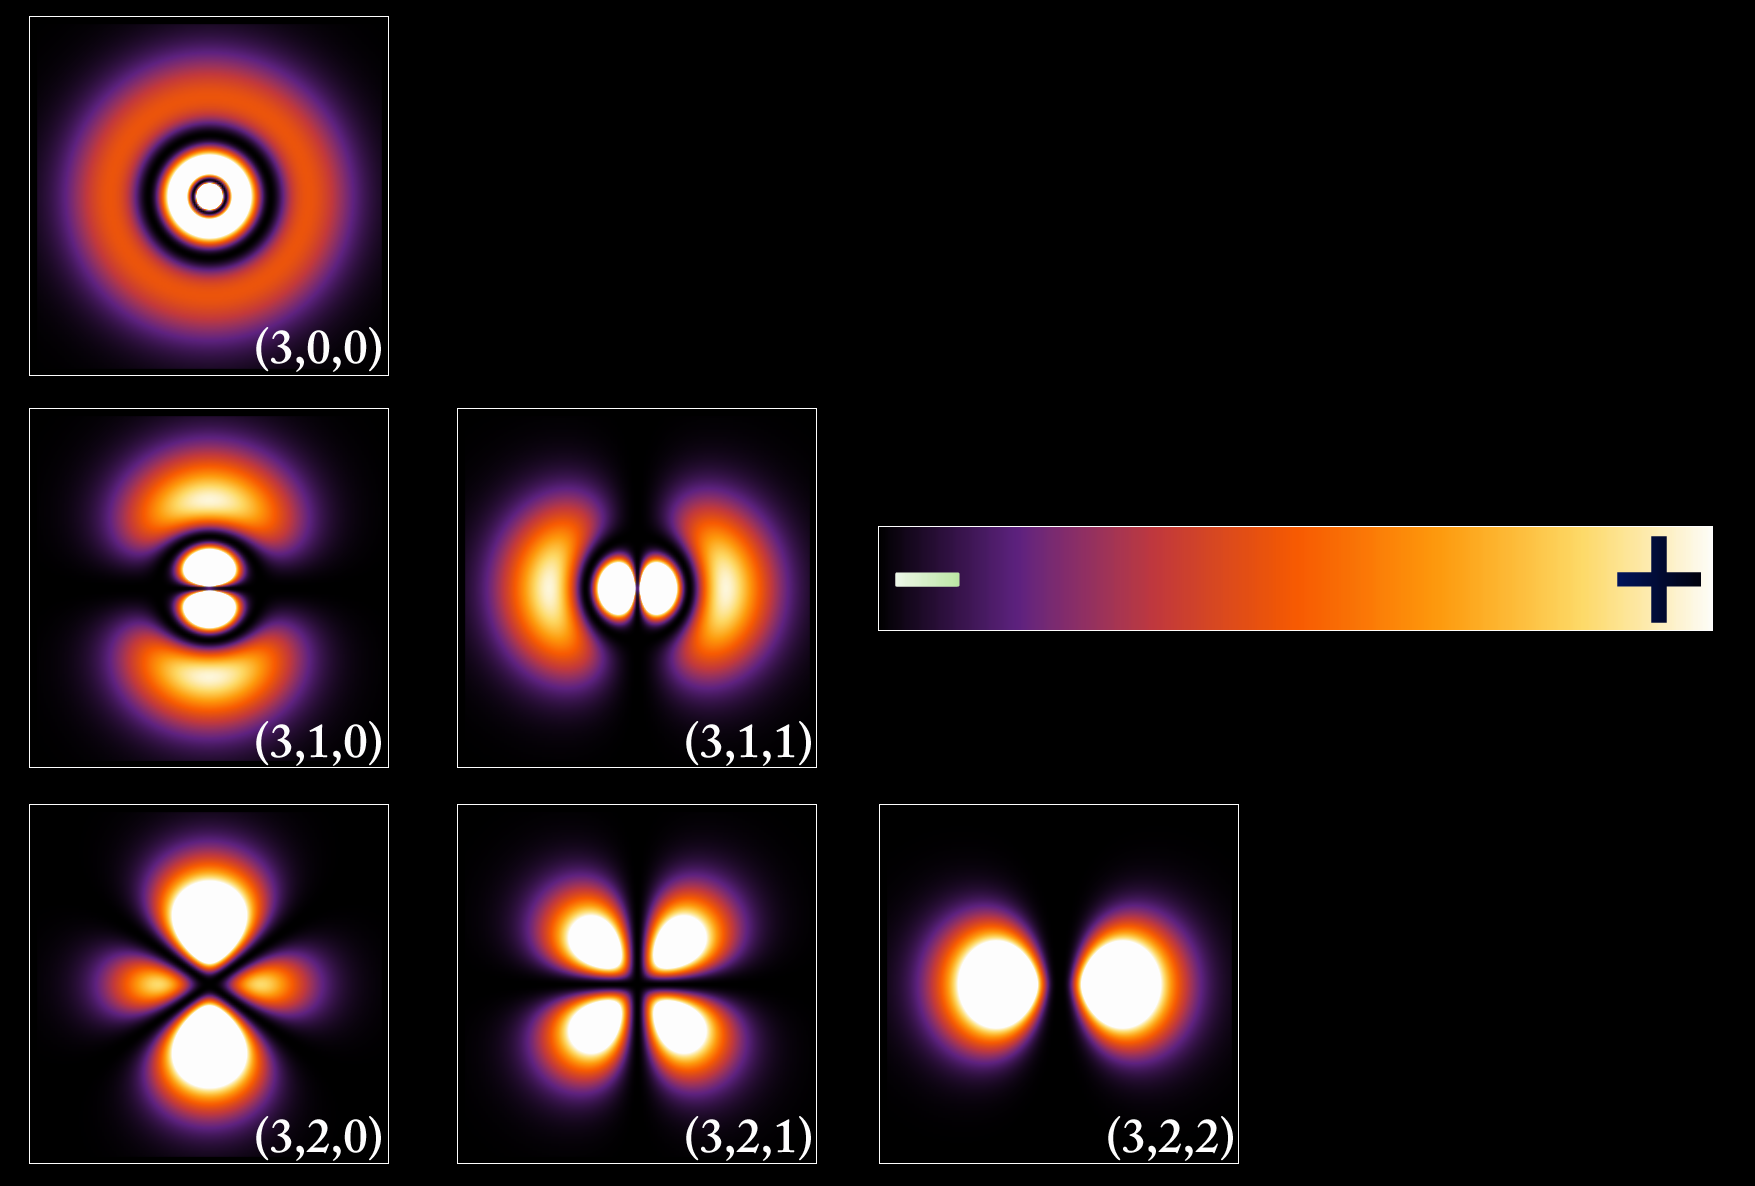
\includegraphics[width = 8.2cm]{Hydrogen_Density_Plots.png}
\caption{Probability density plots for different hydrogen orbital wave functions corresponding to quantum numbers $(n, l, m)$ for $n = 3$. d-wave functions correspond to $l=2$. Note that the probability density is always higher in a region near the nucleus, and has a complicated shape, which will lead to a non-uniform distribution of electronic charge, as opposed to the case of the free electron gas.}
\end{figure}

Experimentally, $d-$electrons of transition metals show a hybrid behavior: sometimes they are accurately described by an ordinary band model, but there are occasions in which the atomic model is better. For example, we see spin wave phenomena in ferromagnetic transition metals, and the susceptibilities of some of these metals depend strongly on temperature. This is characteristic of an atomic (Heisenberg) model. On the other hand, the $d-$electrons contribute significantly to the low temperature specific heat and sometimes the magnetic moments per atom of some transition metal ferromagnets are not integer multiples of the Bohr magneton. This is characteristic of band theory. Our theory of correlations should describe this balance between band-like and atomic-like behavior.

The atomic picture of a solid consists of an electron gas where ions are immersed. The ions then interact in much the same way as they do in salts. This extreme scenario is surely not even close to the true state of affairs since the number of $d-$electrons per atom is in general not an integer. This motivates us to introduce a less restrictive model, which is not too far from the atomic model. We shall assume that while $d-$electrons still have some band motion, they are strongly correlated with each other so that the metal retains some atomic-like behavior. The correlations between electrons on different atoms are likely much weaker and we neglect them.

Let us now look at an example of the aforementioned circumstance. Take a partially filled $d-$band of non-interacting electrons. The spin of any given atom in the solid is just the total spin of all electrons on that atom. It fluctuates both in magnitude and in direction, with a characteristic time that depends on how frequently $d-$electrons hop (in the loose quantum mechanical sense). We can estimate the time interval between $d-$electron hopping events between atoms as a being of the order $\frac{\hbar}{\Delta}$, where $\Delta$ is the $d-$electron bandwidth. The spin can thus be thought of as being associated to each individual moving $d-$electron.

How do the electron interactions affect this picture? We start by recalling Hund's rule: the nature of the  interactions between atoms leads to an alignment of the spins on each atom. Since the atomic picture seems to prevail in our metal, we have reason to expect a similar effect to occur. An atom with a total spin in some direction at a given time will tend to attract electrons with the spin on that direction and repel those with opposite spin. This mechanism makes it unlikely for the spin of an atom to change much over time.

If the interactions between atoms are strong enough, the correlations become considerable, and to state it more precisely, the total spin of an atom will persist for a time that is long compared with the $d-$electron hopping time. Note that it is not the localization of the electrons that causes the spin state of the atom to persist. The specific electrons belonging to a given atom change all the time as long as their spin is consistent with the total spin requirement imposed by Hund's rule. For strong enough correlations, we may think of the spin as being associated to each atom, which opens up the possibility to describe the system using an atomic Heisenberg model.

In short, electrons hop rapidly from atom to atom in a band-like fashion, but their motion is correlated in such a way that atomic characteristics emerge. The extent of atomic behavior depends, of course, on the strength of the interaction.

A theory of electron correlations in a narrow energy band should reduce to an atomic model in the appropriate limit, for example atoms that are so far apart on a lattice that they interact only very weakly. Although we always keep in mind that we are focusing on $d-$electrons, we shall consider $s-$electrons in what follows for the sake of simplicity. The important conclusions will not differ significantly. We will use the atomicity of the electronic distribution to introduce an approximate representation of the electron interaction. It turns out that this representation is mathematically much simpler to handle than the Coulomb interaction itself.

\subsection{Hubbard Hamiltonian}\paragraph{}

Imagine a partially filled narrow $s-$band with $n$ electrons per atom. Suppose you have obtained Bloch wave functions $\psi_{\bm k}$ corresponding to energies $\varepsilon_{\bm k}$ by solving the Schr\"odinger equation for some spin-independent mean field Hartree-Fock potential that accounts for the average interaction of the $s-$band electrons with electrons on other bands, and the interaction with the other $s-$electrons. The electrons on the band evolve according to the Hamiltonian (in a suitable unit system):

\begin{equation}\label{eq:startingHamiltonian}
\begin{split}
&\mathcal{H} = \sum_{\bm k \sigma} \varepsilon_{\bm k} c_{\bm k \sigma}^\dagger c_{\bm k \sigma} + \\
&\frac{1}{2} \sum_{ \substack{\bm k_1 \bm k_2 \\ \bm k_1' \bm k_2' \\ \sigma_1 \sigma_2 } } \left\langle \bm k_1 \bm k_2 \bigg| \frac{e^2}{r} \bigg| \bm k_1' \bm k_2' \right\rangle 
 c_{\bm k_1 \sigma_1}^\dagger c_{\bm k_2 \sigma_2}^\dagger c_{\bm k_2' \sigma_2} c_{\bm k_1' \sigma_1} \\
 &- \sum_{ \substack{\bm k \bm k' \\ \sigma} } \bigg[ 2 \left\langle \bm k \bm k' \bigg| \frac{e^2}{r} \bigg| \bm k \bm k' \right\rangle - \left\langle \bm k \bm k' \bigg| \frac{e^2}{r} \bigg| \bm k' \bm k \right\rangle \bigg] \nu_{\bm k'} c_{\bm k \sigma}^\dagger c_{\bm k \sigma} ,
\end{split}
\end{equation}
where the $\bm k-$sums run over the first Brillouin zone. The integrals are defined by

\begin{equation}\label{eq:integrals}
\begin{split}
&\left\langle \bm k_1 \bm k_2 \bigg| \frac{e^2}{r} \bigg| \bm k_1' \bm k_2' \right\rangle \equiv V^{\bm k_1 \bm k_2}_{\bm k_1' \bm k_2'}  =  \\
&e^2 \int \frac{\psi_{\bm k_1}^\star (\bm x) \psi_{\bm k_1'} (\bm x) \psi_{\bm k_2}^\star (\bm x') \psi_{\bm k_2'}(\bm x') }{| \bm x - \bm x' |} d\bm x d\bm x'
\end{split}
\end{equation}

The first term represents the band energies of the electrons and the second term represents the interactions among them. The last term subtracts the potential energy of the electrons in the part of the Hartree-Fock field due to the electrons of the $s-$band itself. This term ensures that we do not count the interactions of the electrons of the band twice: the Hartree-Fock field that specifies $\varepsilon_{\bm k}$ is computed taking into account these interactions, so if we didn't subtract the last term, we would count the energy of these interactions twice since they reappear in the second term. Furthermore, we assume that up and down spins are occupied equally, and $\nu_{\bm k}$ are the occupation numbers of the states of the band in the Hartree-Fock calculation. 

The term that we subtract in equation ($\ref{eq:startingHamiltonian}$) corresponds to the part of the interaction term which is already accounted for by the first diagonal mean field term. Thus, it corresponds to the mean field expansion of the interaction term (i.e. the second term), which is generically written

\begin{equation}
V_{\text{int}} = \frac{1}{2} V^{\nu\mu}_{\nu'\mu'} c_\nu^\dagger c_\mu^\dagger c^{\mu'} c^{\nu'}
\end{equation}

We start by noting that in mean field, this quartic term becomes a sum of all possible 2-body terms (note that terms of the type $\left\langle cc \right\rangle$ and $\left\langle c^\dagger c^\dagger \right\rangle$ vanish.

\begin{equation}\label{eq:c_mft}
\begin{split}
&c_\nu^\dagger c_\mu^\dagger c_{\mu'} c_{\nu'} \approx - \left\langle c_\nu^\dagger c_{\mu'} \right\rangle  c_{\mu}^\dagger c_{\nu'} - \left\langle c_{\mu}^\dagger c_{\nu'} \right\rangle c_{\nu}^\dagger c_{\mu'} + \\
&+ \left\langle c_{\nu}^\dagger c_{\nu'} \right\rangle  c_{\mu}^\dagger c_{\mu'} + \left\langle c_{\mu}^\dagger c_{\mu'} \right\rangle  c_{\nu}^\dagger c_{\nu'} ,
\end{split}
\end{equation}
where we ignored the constant terms which are unimportant in the Hamiltonian. This Hartree-Fock mean field approximation is slightly tricky to show. It requires one to be precise about what the meaning of the mean field approximation is in terms of creation and annihilation operators. In mean field theory, we assume that the operator

\begin{equation}
\rho_{\mu\mu'} = c_{\mu}^\dagger c_{\mu'}
\end{equation}
is close to its average, so that we neglect second order terms in the fluctuations $\delta \rho_{\mu\mu'}$, i.e. $\rho_{\mu\mu'}$ is \say{large} only when its average is nonzero, otherwise it is negligibly small. Thus, for most combinations of indices, this operator will vanish. We follow the usual mean field procedure of writing the original operator as a deviation plus an average

\begin{equation}\label{eq:hartree}
c_{\nu}^\dagger \bigg( c_\mu^\dagger c_{\mu'} - \left\langle c_\mu^\dagger c_{\mu'} \right\rangle \bigg) c_{\nu'} + c_{\nu}^\dagger c_{\nu'} \left\langle c_\nu^\dagger c_{\nu'} \right\rangle
\end{equation}

Then we note that if $\nu' \neq \mu$, we can commute $c_{\nu'}$ with the parenthesis. But this is true except in a set of measure zero. In the thermodynamic limit $N \rightarrow \infty$, the number of allowed $\bm k$-states is very large, and if we imagine the set of possible $\bm k$-states to be continuous, then the commutation becomes exact. Repeating the procedure of writing (\ref{eq:hartree}) with $c_\nu^\dagger c_{\nu'} - \left\langle c_\nu^\dagger c_{\nu'} \right\rangle + \left\langle c_\nu^\dagger c_{\nu'} \right\rangle $, we obtain

\begin{equation}
\begin{split}
&\underbrace{\big( c_\nu^\dagger c_{\nu'} - \left\langle c_\nu^\dagger c_{\nu'} \right\rangle \big) \big( c_\mu^\dagger c_{\mu'} - \left\langle c_\mu^\dagger c_{\mu'} \right\rangle \big)}_{\propto \, \delta \rho_{\mu\mu'} \, \delta \rho_{\nu\nu'} \rightarrow 0} + c_\nu^\dagger c_{\nu'} \left\langle c_\mu^\dagger c_{\mu'} \right\rangle \\
&+ c_\mu^\dagger c_{\mu'} \left\langle c_\nu^\dagger c_{\nu'} \right\rangle - \left\langle c_\mu^\dagger c_{\mu'} \right\rangle \left\langle c_\nu^\dagger c_{\nu'} \right\rangle
\end{split}
\end{equation}

But this result is not complete. This is only the so called Hartree or direct term. Due to identical nature of the interacting electrons, we must consider an analogous contribution for $\left\langle c_\nu^\dagger c_{\mu'} \right\rangle$ finite. We start by exchanging the first two operators: 

\begin{equation}
c_\nu^\dagger c_\mu^\dagger c_{\mu'} c_{\nu'} = - c_\mu^\dagger c_\nu^\dagger c_{\mu'} c_{\nu'}
\end{equation}
Then we proceed in exactly the same manner as before. The result is analogous, but a minus sign appears and we must switch $\mu \leftrightarrow \nu$:

\begin{equation}
- c_\mu^\dagger c_{\nu'} \left\langle c_\nu^\dagger c_{\mu'} \right\rangle \\
- c_\nu^\dagger c_{\mu'} \left\langle c_\mu^\dagger c_{\nu'} \right\rangle + \left\langle c_\nu^\dagger c_{\mu'} \right\rangle \left\langle c_\mu^\dagger c_{\nu'} \right\rangle
\end{equation}

Ignoring the constant terms of the type $\left\langle c^\dagger c \right\rangle \left\langle c^\dagger c \right\rangle$, we recover equation (\ref{eq:c_mft}).

Now we can simply substitute the mean field expansion of equation (\ref{eq:c_mft}) in the second term to  obtain the last term that is subtracted in equation (\ref{eq:startingHamiltonian}) (we omit the boldface on the $\bm k_i^{(')}$'s solely in the following equation, but keep in mind that they are vectors):

\begin{equation}\label{eq:mean_field}
\begin{split}
&\frac{1}{2} \sum_{\substack{ k_1 k_2 k_1' k_2' \\ \sigma_1 \sigma_2} } V^{k_1 k_2}_{k_1' k_2'} \bigg( - \underbrace{\left\langle c_{k_1 \sigma_1}^\dagger c_{k_2' \sigma_2} \right\rangle}_{\delta_{k_1 k_2'} \delta_{\sigma_1 \sigma_2} \nu_{k_1} } c_{k_2 \sigma_2}^\dagger c_{k_1' \sigma_1} \\
& - \underbrace{\left\langle c_{k_2 \sigma_2}^\dagger c_{k_1' \sigma_1}  \right\rangle}_{\delta_{k_2 k_1'} \delta_{\sigma_1 \sigma_2} \nu_{k_2} } c_{k_1 \sigma_1}^\dagger c_{k_2' \sigma_2} + \underbrace{\left\langle c_{k_1 \sigma_1}^\dagger c_{k_1' \sigma_1} \right\rangle}_{\delta_{k_1 k_1'} \nu_{k_1} } c_{k_2 \sigma_2}^\dagger c_{k_2' \sigma_2}  \\
& + \underbrace{\left\langle c_{k_2 \sigma_2}^\dagger c_{k_2' \sigma_2} \right\rangle}_{\delta_{k_2 k_2'} \nu_{k_2} } c_{k_1 \sigma_1}^\dagger c_{k_1' \sigma_1} \bigg)\\
\end{split}
\end{equation}

In the language of Hartree Fock theory, the first two terms give the exchange term, and the last two terms the direct term. Apart from the $\frac{1}{2}$ factor, the term in (\ref{eq:mean_field}) becomes

\begin{equation}
\begin{split}
&- \sum_{\substack{k_1 k_2 \\ k_1' \sigma_1}} V_{k_1' k_1}^{k_1 k_2} \nu_{k_1} c_{k_2 \sigma_1}^\dagger c_{k_1' \sigma_1}  - \sum_{\substack{k_1 k_2 \\ k_2' \sigma_1}} V_{k_2 k_2'}^{k_1 k_2} \nu_{k_2} c_{k_1 \sigma_1}^\dagger c_{k_2' \sigma_1} \\
&+ \sum_{\substack{k_1 k_2 k_2' \\ \sigma_1 \sigma_2}} V_{k_1 k_2'}^{k_1 k_2} \nu_{k_1} c_{k_2 \sigma_2}^\dagger c_{k_2' \sigma_2}  + \sum_{\substack{k_1 k_2 k_1' \\  \sigma_1 \sigma_2}} V_{k_1' k_2'}^{k_1 k_2} \nu_{k_2} c_{k_1 \sigma_1}^\dagger c_{k_1' \sigma_1} \\
&= \sum_{k_1 k_2 \sigma_1} \bigg( 4 V_{k_1 k_2}^{k_1 k_2} - 2  V_{k_2 k_1}^{k_1 k_2}  \bigg) \nu_{k_2} c_{k_1 \sigma_1}^\dagger c_{k_1 \sigma_1}
,
\end{split}
\end{equation}
where we used momentum conservation to eliminate a $k'$-sum. Moreover, we used that the sum on spin ($\pm 1/2$) on the last two terms gives factors of 2 , since the interaction is spin independent and thus no spin-dependent term remains after we use momentum conservation. Making $k_1 \rightarrow k , \, k_2 \rightarrow k', \, \sigma_1 \rightarrow \sigma$, and recalling the definition in equation (\ref{eq:integrals}), we obtain the result we sought.

Now consider the Wannier functions

\begin{equation}
\phi(\bm x) = N^{-1/2} \sum_{\bm k} \psi_{\bm k} (\bm x) , 
\end{equation}
where $N$ is the number of atoms. We may write $\psi_{\bm k}$ as a  combination of these Wannier functions localized at each atom.

\begin{equation}
\psi_{\bm k} (\bm x) = N^{-1/2} \sum_i e^{i \bm k \cdot \bm R_i} \phi (\bm x - \bm R_i) ,
\end{equation}
where the sum runs over all atomic positions $\bm R_i$. Introducting the annihilation (creation) operators of an electron of spin $\sigma$ in the orbital state $\phi (\bm x - \bm R_i)$ (at site $i$), $c_{i\sigma}^{(\dagger)}$, we may write

\begin{equation}
c_{\bm k \sigma}^{(\dagger)} = N^{-1/2} \sum_i e^{i \bm k \cdot \bm R_i} c_{i\sigma}^{(\dagger)}
\end{equation}

Thus, the Hamiltonian becomes 

\begin{equation}
\begin{split}
&\mathcal{H} = \sum_{\substack{ i j \\ \sigma} } K_{ij} c_{i \sigma}^\dagger c_{j \sigma} + \\
&\frac{1}{2} \sum_{\substack{i j k l \\ \sigma \sigma'} }\left\langle i j \bigg| \frac{e^2}{r} \bigg| k l \right\rangle 
 c_{i \sigma}^\dagger c_{j \sigma'}^\dagger c_{l \sigma'} c_{ k \sigma} \\
 &- \sum_{\substack{ijkl \\ \sigma }} \bigg[ 2 \left\langle i j \bigg| \frac{e^2}{r} \bigg| k l \right\rangle - \left\langle i j \bigg| \frac{e^2}{r} \bigg| l k \right\rangle \bigg] \nu_{j l} c_{i \sigma}^\dagger c_{ k \sigma} ,
\end{split}
\end{equation}
where

\begin{equation}\label{eq:hopping_matrix}
K_{ij} = N^{-1} \sum_{\bm k} \varepsilon_{\bm k} e^{i \bm k \cdot ( \bm R_i - \bm R_j )},
\end{equation}
and

\begin{equation}
\nu_{j l} = N^{-1} \sum_{\bm k} e^{i \bm k \cdot ( \bm R_j - \bm R_l) }
\end{equation}

Now comes the crucial approximation. For a narrow energy band, the Wannier functions $\phi$ nearly coincide with atomic $s-$functions. For small bandwidth these $s-$functions form an atomic shell whose radius is small compared with the spacing between atoms (or lattice constant). Thus, the integral $U = \left\langle i i \big| e^2 / r \big| i i \right\rangle$ should be much larger than all other integrals. This suggests the seemingly crude approximation of neglecting all other integrals. It turns out that this approximation is not so radical as it could seem at first sight since the other integrals are indeed much smaller than $U$. In fact, they are smaller by about two orders of magnitude. We end up with

\begin{equation}
\mathcal{H} = \sum_{i, j, \sigma} K_{ij} c_{i\sigma}^\dagger c_{j\sigma} + \frac{U}{2} \sum_{i\sigma} n_{i\sigma} n_{i, -\sigma} - U \sum_{i, \sigma} \nu_{i, i} n_{i, \sigma}
\end{equation}
where $n_{i\sigma} = c_{i\sigma}^\dagger c_{i\sigma}$. Note that $\nu_{i, i} = N^{-1} \sum_{\bm k} \nu_{\bm k} = n/2$, which means that the last term is constant and may be dropped. Now, the hopping matrix $\bm K$ should be found by inverse Fourier transforming the dispersion relation $\varepsilon_{\bm k}$.

In general, we have a well defined crystal wavevector that depends on the symmetry of the lattice, which may be written as the Fourier transform

\begin{equation}
\left| \bm k \right\rangle \equiv \frac{1}{N} \sum_{\bm r} e^{i\bm k \cdot \bm r} \left| \bm r \right\rangle
\end{equation}

Recalling the form of the hopping Hamiltonian

\begin{equation}
\mathcal{H}_{\text{hop}} = - \sum_{\bm r \bm r'} K (\bm r - \bm r') \left| \bm r' \right\rangle \left\langle \bm r \right|
\end{equation}
we can obtain the dispersion relation.

\begin{equation}
\begin{split}
- \mathcal{H}_{\text{hop}} \left| \bm k \right\rangle &= \frac{1}{\sqrt{N}} \sum_{\bm r \bm r'} K ( \bm r - \bm r' ) e^{i \bm k \cdot \bm r} \left| \bm r' \right \rangle \\
&= \frac{1}{\sqrt{N}} \bigg( \sum_{\bm R} K(\bm R) e^{i\bm k \cdot \bm R} \bigg) \bigg( \sum_{\bm r'} e^{i\bm k \cdot \bm r'} \left| \bm r' \right\rangle \bigg) \\
& = \varepsilon_{\bm k} \left| \bm k \right\rangle
\end{split}
\end{equation}
and here we recognize the dispersion relation as the (negative) Fourier transform of the hopping

\begin{equation}
\varepsilon_{\bm k} = - \sum_{\bm R} K(\bm R) e^{i\bm k \cdot \bm R} 
\end{equation}

This gives us an interpretation of the $\bm K$ matrix: given the dispersion relation for a tight binding model, if we take the inverse Fourier transform we obtain the matrix elements $K_{i j}$.

Let's suppose we have the simplest uniform nearest neighbor hopping model. Going back to equation (\ref{eq:hopping_matrix}), and recalling that the sum on $\bm k$ is restricted to the first Brillouin zone, we obtain the usual tight binding result: $K_{\left\langle i j \right\rangle} = - t$ and $0$ otherwise (i.e. $\bm K$ is a very sparse matrix that is only non-zero for $i, j$ nearest neighbors). The Hubbard Hamiltonian is then

\begin{equation}\label{eq:hubbard_hamiltonian}
\mathcal{H} = - t \sum_{\left\langle i, j \right\rangle, \sigma} \bigg(c_{i,\sigma} c_{j,\sigma}^\dagger + c_{j,\sigma} c_{i,\sigma}^\dagger \bigg) + U \sum_{i} n_{i,\uparrow} n_{i\downarrow}
\end{equation}

\subsection{Mott insulators}\paragraph{}

Band theory was found to be flawed soon after it was introduced. The picture it proposes is simple and generally works pretty well. The solutions of the Schr\"odinger for free electrons in a periodic potential $U(\bm r)$, such that $U(\bm r) = U(\bm r + \bm R)$,

\begin{equation}\label{eq:schrodinger}
\bigg[ -\frac{\hbar^2}{2m} \nabla^2 + U(\bm r) \bigg] \psi (\bm r) = \varepsilon \psi (\bm r)
\end{equation}
are given by Bloch's theorem: $\psi_{\bm k} (\bm r) = e^{i\bm k \cdot \bm r} u_{\bm k} (\bm r)$. Replacing this wave function in equation (\ref{eq:schrodinger}), we obtain a differential equation for $u_{\bm k} (\bm r)$, which has in general an infinite number of solutions. We label them with an index $n$, which we call the band index. To each solution there corresponds a function $\varepsilon_{n\bm k}$. The set of these functions is known as the band structure. Since electrons are taken to be independent in band theory, the N-electron eigenstates are obtained by placing an electron in each quantum state. Each state is labelled by its energy $\varepsilon_{n\bm k \sigma}$. Since our model Hamiltonian does not couple spins (via an electron interaction, for example) and assuming there is no external magnetic field and that the system has an inversion center, $\varepsilon_{n\bm k \uparrow} = \varepsilon_{n\bm k \downarrow}$. Note that in general there might energies for which there is no corresponding $\varepsilon_{n\bm k \sigma}$. These form intervals called forbidden bands\footnote{We disregard surface states.}. Thus, the ground state of our model may normally be obtained by filling the energy levels starting from the lowest energy state. Two cases are particularly relevant:
\begin{itemize}
\item Every band is either fully occupied or empty. The first excited state differs from the ground state by $\Delta$, the separation between the last fully occupied band and the first empty band. It is then impossible to induce the motion of the electrons by applying an arbitrarily small voltage. This is what it means to be an \emph{insulator}. Since there $2N$ states per band, this is not possible unless the number of electrons per unit cell is an even integer.
\item One or more of the bands are partially filled. The energy of occupied state of higher energy is named the Fermi energy $\varepsilon_F$. In this case, the separation between the ground state and the first excited state tends to $0$ in the thermodynamic limit, $N \rightarrow \infty$. The system may then respond to infinitesimal excitations, which is the very definition of a metal!
\end{itemize}

Band theory made it made possible to predict whether a solid would be a metal or an insulator.

The success of band theory rests crucially on the independent electron approximation. Thus, it is not surprising that for compounds with strongly correlated electrons the theory might fail. 

\subsection{Effective Hamiltonian}\paragraph{}

\subsection{Exact solutions for simple cases}\paragraph{}

If we relax the condition of fixed number of particles, there is an extra energy term $-\mu N$ in the Hamiltonian (compared to equation (\ref{eq:hubbard_hamiltonian})), where $\mu$ is the chemical potential, and $N$ is the total number of particles. The Hubbard Hamiltonian may then be written as a sum of kinetic, chemical and potential energy terms, respectively:

\begin{equation}\label{eq:hubbard}
\mathcal{H} = \mathcal{H}_K + \mathcal{H}_\mu + \mathcal{H}_V ,
\end{equation}
defined as

\begin{equation}\label{eq:def_energies}
\begin{split}
\mathcal{H}_K &= -t \sum_{\left\langle i, j \right \rangle, \sigma} ( c_{i,\sigma} c_{j,\sigma}^\dagger + c_{j,\sigma}^\dagger c_{i,\sigma} ) \\
\mathcal{H}_\mu &= -\mu \sum_i ( n_{i,\uparrow} + n_{i,\downarrow} ) \\
\mathcal{H}_V &= U \sum_{i} ( n_{i,\uparrow} - \frac{1}{2} ) ( n_{i,\downarrow} - \frac{1}{2} )
\end{split} ,
\end{equation}
where:

\begin{itemize}
\item $i$ and $j$ label sites on the lattice.
\item $c_{i,\sigma}^{(\dagger)}$ is an operator that annihilates (creates) an electron with spin $\sigma$ on site $i$.
\item $n_{i,\sigma}$ is the number operator counting the number of electrons of spin $\sigma$ on site $i$ (either 0 or 1).
\item $t$ is the hopping parameter related to the kinetic energy of the electrons. It is determined by the overlap of the atomic wave functions on neighboring sites $\left\langle i, j \right\rangle$.
\item $U$ is the repulsive Coulomb interaction betweens electrons on the same lattice site. Whenever a site $i$ has two electrons, there is a local repulsion between them corresponding to an energy cost $U n_{i \uparrow} n_{i \downarrow}$. The constant $1/2$ terms serve to recast the Hamiltonian in particle-hole symmetric form.
\item $\mu$ is the chemical potential controlling the electron number (or density).
\end{itemize}

A given physical observable of interest $\mathcal{O}$, such as the spin-spin correlation, or the magnetic susceptibility may be computed formally by

\begin{equation}
\left\langle \mathcal{O} \right\rangle = Tr ( \mathcal{O} \mathcal{P} )
\end{equation}
where

\begin{equation}
\mathcal{P} \equiv \frac{1}{Z} e^{-\beta \mathcal{H} } , \text{ with } Z = Tr ( e^{-\beta \mathcal{H} } )
\end{equation}

The trace is taken over the Hilbert space corresponding to all possible configurations of the lattice occupation. Defining an orthonormal basis of this Hilbert space $\{ | \psi_i \rangle | i = 1, ... D \} $, where $D$ is the dimension of the Hilbert space, the partition function reads

\begin{equation}
Tr ( e^{-\beta \mathcal{H} } )= \sum_i \left\langle \psi_i | e^{-\beta \mathcal{H} } | \psi_i \right\rangle
\end{equation}

There are four possible states at each site in the Hubbard model: $\left| \,\, \right\rangle$, $\left|\uparrow \right\rangle$, $\left|\downarrow\right \rangle$, $\left|\uparrow \downarrow \right\rangle $, corresponding, respectively, to no electron, spin up or spin down electron, and two electrons occupying the site. The potential energy operator acts as follows

\begin{equation}
U (n_{i\uparrow} - \frac{1}{2} ) ( n_{i\downarrow} - \frac{1}{2} ) 
\begin{cases}
\left| \,\, \right\rangle = \frac{U}{4} \left| \,\, \right\rangle \\
\left|\uparrow \right\rangle = -\frac{U}{4} \left|\uparrow \right\rangle \\
\left|\downarrow\right \rangle = -\frac{U}{4} \left|\downarrow\right \rangle \\
\left|\uparrow \downarrow \right\rangle = \frac{U}{4} \left|\uparrow \downarrow \right\rangle \\
\end{cases}
\end{equation}

Singly occupied states ($\left|\uparrow \right\rangle$, $\left|\downarrow\right \rangle$) have lower energy and are thus more likely to occur. They correspond to nonzero magnetization $m = n_{\uparrow} - n_{\downarrow}$, which is favored by the Hubbard interaction $U$. A relevant question is whether or not the spins order in space when $t \neq 0$.

\section{Simulations}\label{hubbQMC}

\subsection{Auxiliary field QMC}\paragraph{}

We will now discuss a numerical method to simulate the Hubbard model: auxiliary field quantum Monte Carlo. This technique allows us to circumvent the sign problem. The sign problem is due to the antisymmetry of the many-electron wave function leading to oscillations in the sign of the quantities that we are interested in measuring. These oscillations deem the algorithm exponentially complex in the size of the system, in general, but it possible to overcome this hurdle for a class of models.

\end{document}